% \documentclass{beamer}
%Information to be included in the title page:
%\title{Moufangové rovina a spinové grupy}
%\author{Dominik Stejskal}
% \institute{Overleaf}
%\date{1. 4. 2022}

% test change after setting up offline backup

\documentclass[9pt]{beamer}

\usepackage{times,color}
\usepackage[czech]{babel}
\usepackage[utf8]{inputenc}
\usepackage{amsmath}
\usepackage[cmtip,all]{xy}
\usepackage[T1]{fontenc}
\usepackage[normalem]{ulem}

\usepackage{mathtools}   % přidal jsem já...
\usepackage[bb=stix]{mathalpha}  % KVŮLI LOWERCASE BBM A PDF/A-2u
\usepackage{todonotes}
\setuptodonotes{inline}  % CUSTOMIZACE TODONOTES
\usepackage{bm}

%%%%%% my own macros section %%%%%%%%%%%%%%%%%%%%%
\newcommand{\R}{\mathbb{R}}
\newcommand{\N}{\mathbb{N}}
\newcommand{\Z}{\mathbb{Z}}
\newcommand{\Q}{\mathbb{Q}}
\newcommand{\q}{\mathbb{q}}
\newcommand{\F}{\mathbb{F}}
\newcommand{\G}{\mathbb{G}}
\newcommand{\e}{\hat{e}}

\newcommand{\probability}[2]{
    \Pr
    \left[ 
    \begin{aligned}
    #1 \mspace{1mu}
    \end{aligned}
    \middle\vert
    \begin{aligned}
    \mspace{2mu} #2
    \end{aligned}
    \right]
}

\newcommand{\poly}{\mathsf{poly}}
\newcommand{\Pgen}{\mathsf{PGen}}
\newcommand{\KGen}{\mathsf{KGen}}
\newcommand{\Com}{\mathsf{Com}}
\newcommand{\Open}{\mathsf{Open}}
\newcommand{\V}{\mathsf{Vrf}}  % verification
\newcommand{\Ext}{\mathsf{Ext}}  % extractor
\newcommand{\Rev}{\mathsf{Rev}}  % revealer
\newcommand{\ck}{\mathsf{ck}}  % commitment key
\newcommand{\negligible}{\approx_{\lambda} 0}
\newcommand{\A}{\mathcal A}  % adversary
\newcommand{\B}{\mathcal B}  % adversary
\newcommand{\RND}{\mathsf{RND}_\lambda}  % random tape
\newcommand{\gp}{\mathsf{gp}}  % group parameters
\newcommand{\Oracle}{\mathcal{O}}  % oracle
\newcommand{\EF}{\mathcal{EF}}  % family of functions
\newcommand{\DF}{\mathcal{DF}}  % family of distributions
\newcommand{\il}{\mathsf{il}}  % input length
\newcommand{\ol}{\mathsf{ol}}  % output length
\newcommand{\ql}{\mathsf{ql}}  % query length
\newcommand{\fpr}{\mathsf{fpr}}  % find polynomial representation
\newcommand{\tofr}{\mathsf{tofr}}  % find polynomial representation
\DeclareMathOperator{\vectorization}{vec}
\newcommand{\Vexpl}{V^\mathsf{expl}}  % explicit verification polynomial
\newcommand{\caseA}{\ensuremath{\mathsf{A}}}
\newcommand{\caseQ}{\ensuremath{\mathsf{Q}}}
\newcommand{\caseX}{\ensuremath{\mathsf{X}}}
\newcommand{\caseXone}{\ensuremath{\mathsf{X.1}}}
\newcommand{\caseXtwo}{\ensuremath{\mathsf{X.2}}}

%%%%%%%%%%%%%%%%%%%%%%%%%%%%%%%%%%%%%%%%%%%%%%%%%%%%%%%%%%%%%%%%%%%%%%%%%

\newtheorem{proposition}{Proposition}
%\newtheorem{theorem}{Theorem}
%\newtheorem{lemma}{Lemma}
%\newtheorem*{example}{Example}
\mode<presentation>
{
  \usetheme{Warsaw}
  \title{On the power of algebraic group models}
  \author{Dominik Stejskal}
  \date{Supervisor: Mgr. Pavel Hubáček, Ph.D.\\ \, \\2 June 2025}
}

%%%%%%%%%%%%%%%%%%%%%%%%%%%%%%%%%%%%%%%%%%%%%%%%%%%%%%%%%%%%%%%%%%%%%%

\begin{document}

\frame{\titlepage}




\begin{frame}
\frametitle{Overview}
\begin{itemize}
\item What are the important things about the thesis
\item etc.
\end{itemize}
\end{frame}


\begin{frame}
\frametitle{Preliminaries}
\begin{itemize}
    \item Security parameter $ \lambda $
    \item Group parameters 
    \[
    \Pgen(1^\lambda) \to \gp = (p, \G_1, \G_2, \G_T, [1]_1, [1]_2, [1]_T, \hat e)
    \]
    \item $ p $ a prime %, $ \F = \Z_p $
    \item $ (\G_1, +) $, $ (\G_2, +) $, $ (\G_T, +) $ cyclic groups of order $ p $
    \item $ \e \colon \G_1 \times \G_2 \to \G_T $ a \textit{pairing}, i.e., a non-degenerate, efficiently computable bilinear map \todo{todo: use only $ a \bullet b $ notation?}
    \item For $ \kappa \in \{ 1, 2, T \} $, $ a \in \F $ and $ \mathbb b \in \F^n $, let $ [a]_\kappa = a[1]_\kappa \in \G_\kappa $, 
    \[ 
    [\mathbb b]_\kappa = [b_1, \dots, b_n]_\kappa = ([b_1]_\kappa, \dots, [b_n]_\kappa) \in \G_\kappa^n
    \]
    \todo{maybe only mention negligible fn when it is used (once)?}
    \item A \textit{negligible function} approaches $ 0 $ faster than any inverse polynomial: $ \phi(\lambda) \negligible $
\end{itemize}
\end{frame}


\begin{frame}
\frametitle{Polynomial Commitment Schemes (PCSs)}
\todo{todo: enlarge, move things around}
    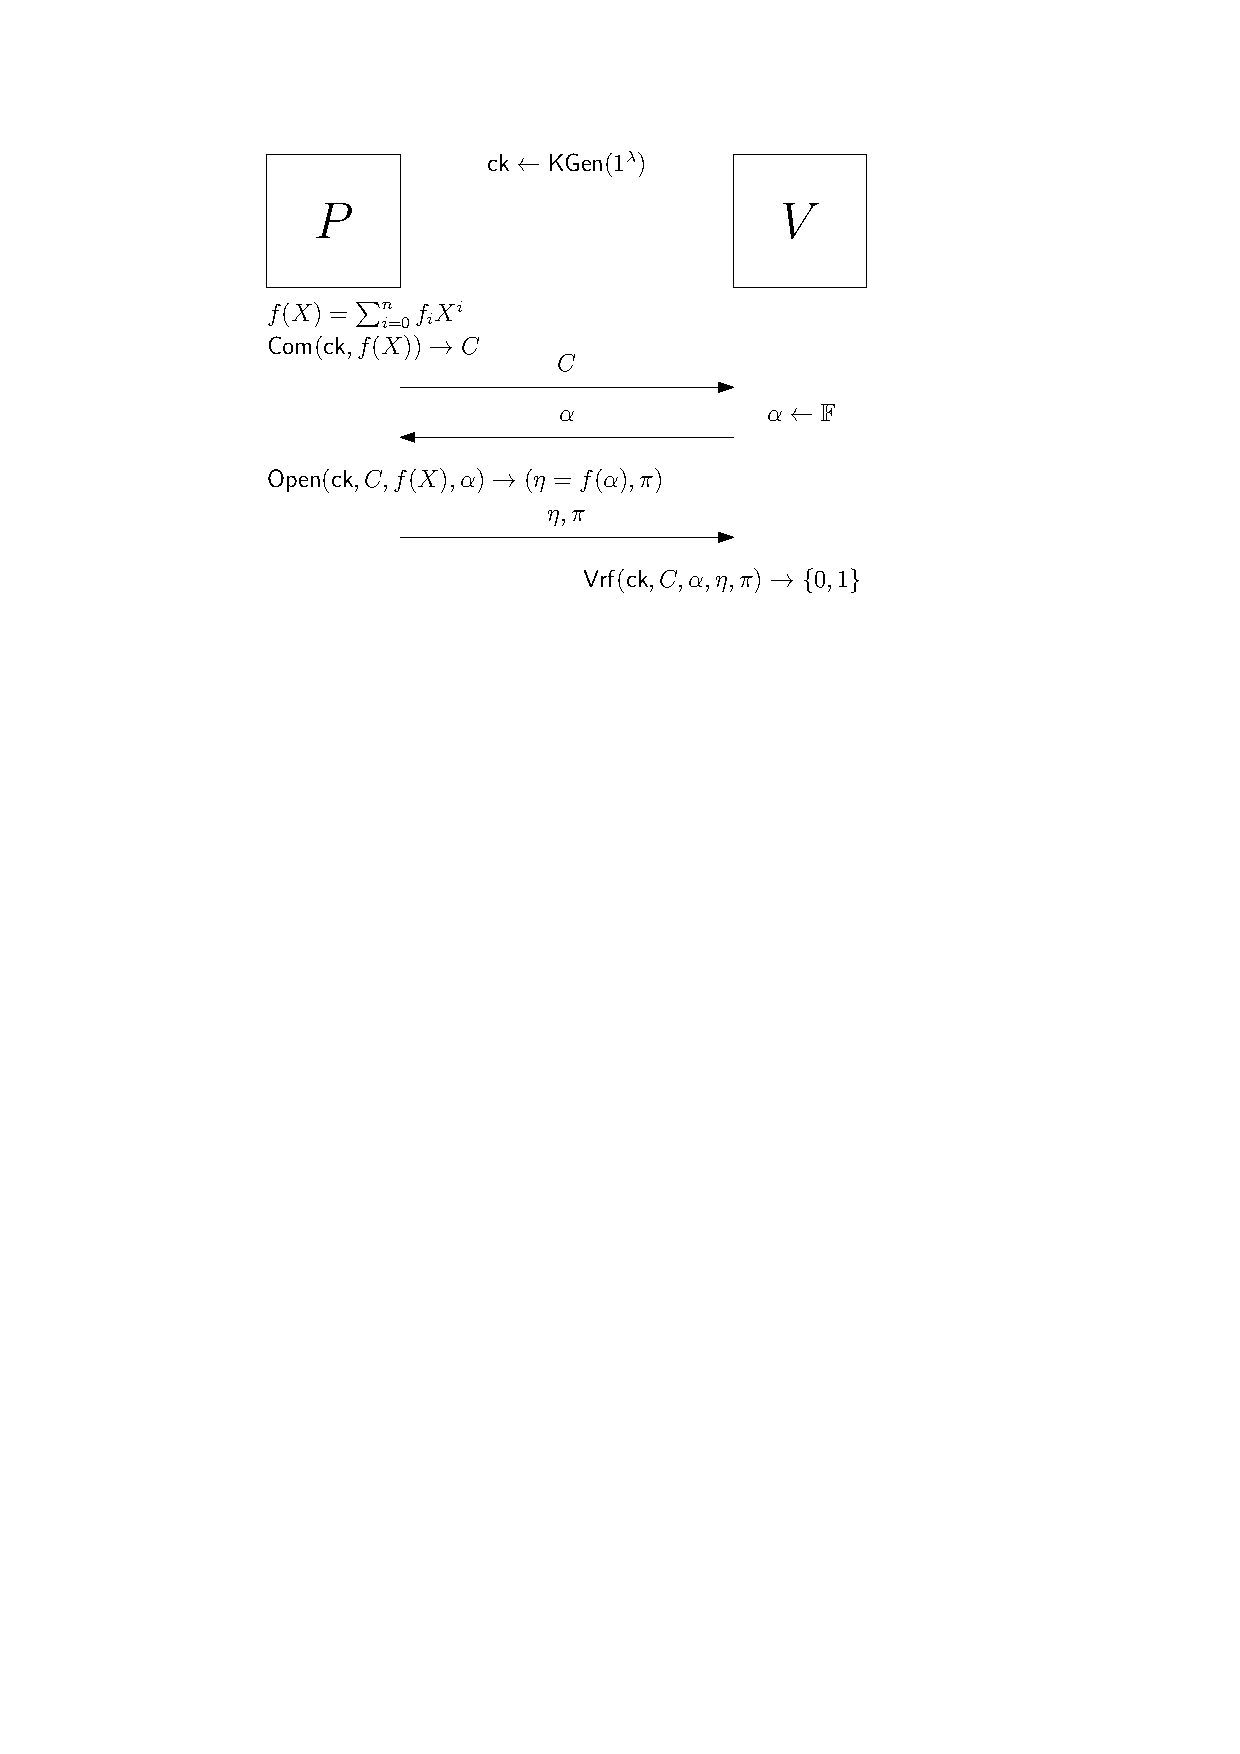
\includegraphics[width=10cm]{pcs-definition.pdf}
\end{frame}


\begin{frame}
\frametitle{Kate-Zaverucha-Goldberg (KZG)}
    
\end{frame}


\begin{frame}
\frametitle{Security properties of PCSs}
\todo{still too long?}
\begin{definition}
    A PCS is \emph{evaluation binding} if for any $ n \in \poly(\lambda) $ and PPT adversary $ \A $, 
    $$
    \probability{
    & \V(\ck, C, \alpha, \eta, \pi) = 1 \; \land \\ 
    & \V(\ck, C, \alpha, \eta', \pi') = 1 \; \land \\ 
    & \; \eta \neq \eta'
    }{
    & \gp \leftarrow \Pgen(1^\lambda); \ck \leftarrow \KGen(\gp, n); \\
    & (C, \alpha, \eta, \pi, \eta', \pi') \leftarrow \A(\ck)
    }
    \negligible.
    $$
\end{definition}
Intuition: it is hard to prove the nonsensical claim that $ \eta = f(\alpha) = \eta' \neq \eta $.
\begin{definition}[informal]
    A PCS is \textit{extractable} if, for every PPT adversary $ \A $, there exists a PPT \textit{extractor} $ \Ext_{\A} $ satisfying the following. If $ \A $'s output passes the PCS verification, then $ \Ext_\A $, given ``access'' to $ \A $, ``extracts'' the committed polynomial $ f(X) $.
\end{definition}
Intuition: a successful prover must be ``thinking of $ f(X) $ in its head''.
\end{frame}


\begin{frame}
\frametitle{Algebraic Group Model}
\todo{do I have to mention GGM?}
\begin{itemize}
    \item Every PPT adversary is \textit{algebraic}:
    $$
    \A(\gp, [\mathbb x_1]_1, [\mathbb x_2]_2) \to (([\mathbb y_1]_1, \bm \gamma_1), ([\mathbb y_2]_2, \bm \gamma_2)),
    $$
    where $ \bm{\gamma}_1 $, $ \bm{\gamma}_2 $ are matrices over $ \F $, and it holds that 
    \begin{equation*}
    \mathbb y_1 = \bm{\gamma}_1 \mathbb x_1, \quad 
    \mathbb y_2 = \bm{\gamma}_2 \mathbb x_2. 
    \end{equation*}
\end{itemize}
\begin{proposition}
    In the AGM, the discrete logarithm assumption and the computational Diffie-Hellman assumption are equivalent.
\end{proposition}
\end{frame}


\begin{frame}
\frametitle{Extractability in the AGM}
\todo{todo: show for KZG...}
Building on the ideas of P.\ Chmel, C.\ Hoffmann and P.\ Hubáček:
\begin{theorem}[informal]
In the AGM, if a ``\textbf{KZG-like}'' PCS is evaluation binding, then it is extractable.
\end{theorem}
Conclusion: the AGM is likely not suitable for proving extractability. 
\end{frame}


\begin{frame}
\frametitle{The end}
Thank you for your attention.
\end{frame}


\end{document}